\section{Elementary Maths}
Should be fairly easy, this section is just so that everyone is one the same page and use the same notation for the rest of the course.
I will go fast as I assume you have already seen this before.
\subsection{Mathematical Objects \& Notations}
\subparagraph{Sets}
\begin{definition}[Sets]
    Unordered list of elements.
\end{definition}
\begin{notation}[Sets]
    $a \in A$, $\{ a, b, c \dots \}$, $\{ e \mid condition \}$, $\emptyset$
\end{notation}
\begin{remark}[Russell Paradox]
    \textit{(digression)}\\
    Need to be careful when defining set: some definitions are pathological.
    
    e.g.: Take $Y = \{x \mid x \not\in x\}$:
    $Y \in Y \iff Y \not\in Y$
\end{remark}

\subparagraph{Types of numbers}
\begin{definition}[Booleans]
    The set of boolean numbers $\B$ is $\{0,1\}$ or sometimes denoted $\{False, True\}$.\\
\end{definition}
\begin{definition}[Naturals]
    The set of natural numbers $\N$ is $\{0,1,2,3,\dots\}$.\\
    N.B.: some countries do not count $0$ as a natural number; but we are in France, so in this course, we will.\\
    N.B.(bis): If we need the naturals without zero, we will use $\N^*$.
\end{definition}
\begin{definition}[Integers]
    The set of integral numbers $\Z$ is $\{0,1,-1,2,-2,3,-3,\dots\}$.\\
    N.B.: If we need only the negative part of the integers, we will use $\Z^-$.
\end{definition}
\begin{definition}[Rationals or Quotients or Fractions]
    The set of natural numbers $\Q$ is $\{\nicefrac{a}{b} \mid a \in \Z, b \in \N^*\}$.\\
\end{definition}
\begin{definition}[Reals]
    The set of real numbers $\R$ is the set of "all numbers you can think of": rational + irrationals (e.g.: roots). 
\end{definition}
Typical diagram:\\
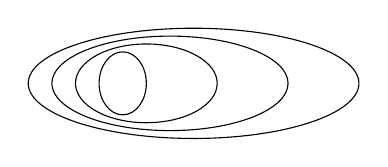
\begin{tikzpicture}
    %ellipses
    \draw (0,1) ellipse (0.3cm and 0.4cm);
    \draw (0.3,1) ellipse (0.9cm and 0.5cm);
    \draw (0.6,1) ellipse (1.5cm and 0.6cm);
    \draw (0.9,1) ellipse (2.1cm and 0.7cm);
    %math
    \draw (0,1) node[anchor=center] {$\N$};
    \draw (0.7,1) node[anchor=center] {$\Z$};
    \draw (1.6,1) node[anchor=center] {$\Q$};
    \draw (2.5,1) node[anchor=center] {$\R$};
\end{tikzpicture}\\
Later, we will see complex numbers.
In computer science, types matter a lot.

\subparagraph{Functions}
\begin{definition}[Functions]
    Assignment from a set to another.
\end{definition}
\begin{notation}[Function]
    $f: X \to Y$, $f(x)=blah$, $f: x \mapsto blah$.
\end{notation}
\begin{question}
    Which ones of these function are well-defined ?
    \begin{itemize}
        \item $f:k\in \{0,1,2,3,4\}\mapsto 24/k\in \N$
        \item $f:k\in \{1,2,3,4\}\mapsto 24/k\in \N$
        \item $f:k\in \{1,2,3,4,5\}\mapsto 24/k\in \N$
        \item $f:k\in \{1,2,3,4\}\mapsto k\in \{1,2\}$
        \item $f:k\in \{1,2,3,4\}\mapsto k\in \{1,2,3,4,5\}$
    \end{itemize}
\end{question}

\subparagraph{Quantifiers}
\begin{notation}[$\forall$]
    For all elements in set, e.g.: $\forall x \in \R, x^2 \geq 0$.
\end{notation}
\begin{notation}[$\exists$]
    There exists an element in set, e.g.: $\exists x \in \R \text{ s.t. } x^2 > 1$.
\end{notation}
\begin{notation}[$\exists !$]
    There exists a unique element in set, e.g.: $\exists ! x \in \R \text{ s.t. } x^2 \leq 0$.
\end{notation}
\begin{question}
    \begin{itemize}
        \item Express "all natural numbers are positive" with quantifiers
        \item Express $\forall x \geq 0, \ \sqrt{x} \geq 0$ in a sentence
    \end{itemize}
\end{question}
\begin{definition}[Subset / Inclusion]
    $X \subseteq Y$ if $\forall x \in X, x \in Y$
\end{definition}
\begin{definition}[Disjoint Sets]
    $X$ and $Y$ are disjoint if $\forall x \in X, x \not\in Y$ (or if $\forall y \in Y, y \not\in X$).
\end{definition}
\begin{definition}[Power Set]
    $\Pow{X} = \{ Y \mid Y \subseteq X \}$\\
    e.g.: $\Pow{\{1,2,3\}}=\{ \emptyset, \{1\},\{2\},\{3\}, \{1,2\},\{1,3\},\{2,3\}, \{1,2,3\} \}$
\end{definition}

\subparagraph{Scalars vs vectors}
1D vs 2D:\vspace{0.2cm}\\
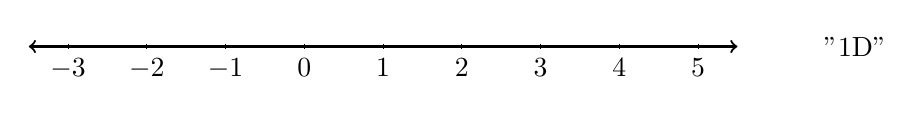
\begin{tikzpicture}
    \draw[thick,<->] (-3.5,0) -- (5.5,0);
    \foreach \x in {-3,-2,-1,0,1,2,3,4,5}
    \draw (\x cm,1pt) -- (\x cm,-1pt) node[anchor=north] {$\x$};
   \draw (7,0) node[anchor=center] {"1D"};
\end{tikzpicture}\\
\begin{tikzpicture}
    \draw[thick,<->] (-1.5,0) -- (3.5,0);
    \draw[thick,<->] (0,-1.5) -- (0,3.5);
    \foreach \x in {-1,1,2,3}
        \draw (\x cm,1pt) -- (\x cm,-1pt) node[anchor=north] {$\x$};
    \foreach \y in {-1,1,2,3}
        \draw (1pt,\y cm) -- (-1pt,\y cm) node[anchor=east] {$\y$};
    \draw (5,1) node[anchor=center] {"2D"};
\end{tikzpicture}\\
To "select" a point in 2D, we need 2 numbers, giving a coordinate.
In 3D, we would need 3 numbers, in 4D, 4 numbers, etc...
\begin{definition}[Cartesian Product]
    $X \times Y = \{ (x,y) \mid x \in X, y \in Y \}$\\
    e.g.: $\{a,b\} \times \{1,2,3\} = \{ (a,1),(a,2),(a,3), (b,1),(b,2),(b,3) \}$\\
    e.g.: $\R \times \R = \{ (x,y) \mid x,y \in \R \}$\\
    Extension: $X_1 \times \dots \times X_n = \prod_{k=1}^n X_k$
\end{definition}
Moving from one point to another gives a "translation".
Again, we need ad many numbers as there are dimensions.
Typically, we denote points horizontally, and vectors vertically.

\subsection{Axioms}
Here $ \star $ and $ \dagger $ will operations.
\begin{definition}[Associativity]
    $\star$ is associative if $\forall x,y,z, \ (x \star y) \star z = x \star (y \star z)$
\end{definition}
\begin{definition}[Commutativity]
    $\star$ is associative if $\forall x,y, \ (x \star y) = y \star x$
\end{definition}
\begin{definition}[Identity]
    $1_{\star}$ is identity for $\star$ if $\forall x, \ 1_{\star} \star x = x \star 1_{\star} = x$
\end{definition}
\begin{definition}[Annihilator]
    $0_{\star}$ is annihilator for $\star$ if $\forall x, \ 0_{\star} \star x = x \star 0_{\star} = 0_{\star}$
\end{definition}
\begin{definition}[Distributivity]
    $\star$ is distributive over $\dagger$ if $\forall x,y,z \ x \star (y \dagger z) = (x \star y) \dagger (x \star z)$
\end{definition}


 of $\land$ over $\lor$:  $x \land (y \lor z) = (x \land y) \lor (x \land z)$
\begin{question}
    \begin{itemize}\textit{(make a table)}
        \item Which of these are commutative: addition, subtraction, multiplication, division, power?
        \item Which of these are associative: addition, subtraction, multiplication, division, power?
        \item What is identity for: addition, subtraction, multiplication, division, power?
        \item What is annihilator for: addition, subtraction, multiplication, division, power?
    \end{itemize}
\end{question}
\begin{question}
    \begin{itemize}
        \item Think of an operation that is commutative, but not associative
        \item Think of an operation that is associative, but not commutative
    \end{itemize}
\end{question}


\subsection{Boolean algebra}
\textit{The reason we'll do some is because of it's application to programming, in particular to conditions ('if' blocks and 'while' loops).}
\subparagraph{Basic operators}
\begin{definition}[Conjunction]
    $x \land y = xy$
\end{definition}
\begin{definition}[Intersection]
    $X \cap Y = \{ z \mid (z \in X) \land (z \in Y) \}$
\end{definition}
\begin{remark}[Disjoint Sets and Intersection]
    Disjoint sets have empty intersection.
\end{remark}
\begin{definition}[Disjunction]
    $x \lor y = \min(x+y,1)$
\end{definition}
\begin{definition}[Union]
    $X \cup Y = \{ z \mid (z \in X) \lor (z \in Y) \}$
\end{definition}
\begin{definition}[Negation]
    $\lnot: 0,1 \mapsto 1,0$
\end{definition}
\begin{definition}[Set minus / Complement]
    $X \setminus Y = \{ x \in X \mid \lnot (x \in Y) \}$
\end{definition}
[Draw diagrams]
\begin{question}
    Selecting points outside a given region.
\end{question}
\subparagraph{Basic properties}
\begin{property}[Boolean algebra matching ordinary algebra]
    Same laws as ordinary algebra when one matches up $\lor$ with addition and $\land$ with multiplication.
    \begin{itemize}
        \item Associativity of $\lor$: $x \lor (y \lor z) = (x \lor y) \lor z$
        \item Associativity of $\land$: $x \land (y \land z) = (x \land y) \land z$
        \item Commutativity of $\lor$: $x \lor y  = y \lor x$
        \item Commutativity of $\land$: $x \land y  = y \land x$
        \item Distributivity of $\land$ over $\lor$:  $x \land (y \lor z) = (x \land y) \lor (x \land z)$
        \item $0$ is identity for $\lor$: $x \lor 0  = x$
        \item $1$ is identity for $\land$: $x \land 1  = x$
        \item $0$ is annihilator for $\land$: $x \land 0  = 0$
    \end{itemize}
\end{property}
\begin{property}[Boolean algebra specific properties]
    The following laws hold in Boolean algebra, but not in ordinary algebra: 
    \begin{itemize}
        \item Idempotence of $\lor$: $x \lor x = x$
        \item Idempotence of $\land$: $x \land x = x$
        \item Absorption of $\lor$ over $\land$: $x \lor (x \land y)  = x \land y$
        \item Absorption of $\land$ over $\lor$: $x \land (x \lor y)  = x \lor y$
        \item Distributivity of $\lor$ over $\land$:  $x \lor (y \land z) = (x \lor y) \land (x \lor z)$
        \item $1$ is annihilator for $\lor$: $x \lor 1 = 1$
    \end{itemize}
\end{property}
\begin{property}[De Morgan Laws]
    $\lnot (x \land y) = \lnot x \lor \lnot y$
    and
    $\lnot (x \lor y) = \lnot x \land \lnot y$
\end{property}
\begin{proof}
    Truth-tables; prove De Morgan, others as exercise (or just believe me)
\end{proof}

\subparagraph{Other operators}
\begin{definition}[Exclusive Or]
    $x \oplus y$
\end{definition}
\begin{definition}[Implication]
    $x \implies y$
\end{definition}
\begin{property}[Implication and Inclusion]
    If $\forall x \in X, P_1(x) \implies P_2(x)$, then $\{ x \in X \mid P_1(x) \} \subset \{ x \in X \mid P_2(x) \}$.
\end{property}
\begin{proof}
    Trivial.
\end{proof}
\begin{definition}[If and only if]
    $x \iff y$
\end{definition}
\begin{question}
    Express in terms of and, or, not:
    \begin{itemize}
        \item $\oplus$
        \item $\implies$
        \item $\impliedby$
        \item $\iff$
    \end{itemize}
    Write 1st and 2nd digit of addition of 3 binary numbers $a$, $b$, $c$.
\end{question}

\subparagraph{Negation of quantified propositions}
\begin{property}[Negation of $\forall$]
    $\lnot \forall x\in X, P(x) = \exists x\in X, \lnot P(x)$
\end{property}
\begin{property}[Negation of $\exists$]
    $\lnot \exists x\in X, P(x) = \forall x\in X, \lnot P(x)$
\end{property}
\begin{notation}[Quantifiers and the empty set]
    $\forall x \in \emptyset, \ \dots$ is true ;
    $\exists x \in \emptyset, \ \dots$ is false
\end{notation}
\begin{question} Negate the following
    \begin{itemize}
        \item $\forall x \in \R, \ \exists n \in \N \text{ s.t. } n > x$
        \item ($x_n \to x$): $\forall \epsilon>0, \exists N \in \N \text{ s.t. } \forall n>N, \abs{x_n-x}<\epsilon$
    \end{itemize}
\end{question}



\subsection{Proofs}
Proofs play a major role in mathematics.
Except axioms, every statement needs a proof to be valid.
There are a 4 common approaches to prove a statement:
\paragraph{Direct proof}
This techniques consists of just going straight in and aiming at the statement you want.
\begin{property}[Archimedian Property]
    For any real number, there exists an integer even greater.\\
    That is $\forall x \in \R, \exists n \in \N \text{ s.t. } x<n$.
\end{property}
\begin{proof}
    Let $n = \floor{x}+1$: then $x-1<\floor{x}$ so $x<\floor{x}=n$.
\end{proof}
\paragraph{Splitting cases}
This techniques consists splitting the statement to prove in several easier ones.
\begin{property}
    For any $n \in \Z$, $n$ and $n^2$ share the same parity.
\end{property}
\begin{proof} We split into 2 cases: $n$ even and $n$ odd:
    \begin{itemize}
        \item Suppose $n$ is even: $n=2k$ so $n^2=4k^2=2(2k^2)$, i.e. $n^2$ is even.
        \item Suppose $n$ is odd: $n=2k+1$ so $n^2=4k^2+4k+1=2(2k^2+2k)+1$, i.e. $n^2$ is odd.
    \end{itemize}
\end{proof}
\paragraph{Contradiction}
This techniques consists in assuming the opposite of what you want, deriving a contradiction (both $P$ and $\lnot P$), then conclude the opposite of what was assumed.
\begin{property}
    $\sqrt{2} \not\in \Q$
\end{property}
\begin{proof}
    Suppose $\sqrt{2} \in \Q$: then there are $a,b \in \N$ such that $\sqrt{2} = \nicefrac{a}{b}$.
    Moreover, we can take $a$ and $b$ so that they have no common divisors.
    Now, we have $2b^2 = a^2$. So $a^2$ is even, so $a$ is even, let $a = 2a'$.
    Then, $2b^2 = 4a'^2$ so $b^2 = 2a'^2$. Thus, $b^2$ is even, so $b$ is even.
    Both $a$ and $b$ are divisible by $2$, which contradicts them having no common divisors.
    Finally, we conclude our initial assumption was wrong, so $\sqrt{2} \not\in \Q$.
\end{proof}
\paragraph{Induction}
This techniques is only applicable if we wish to prove a statement for all natural numbers.
The idea is similar to domino: each statement will imply the next one.
Mathematically, if $P(n)$ are statements ($n \in \N$), we give 2 proofs:
First, that $P(0)$ is true.
Then, that $P(n) \implies P(n+1)$.
\begin{property}
    $\forall n \in \N, \ \sum_{k=0}^{n} k = \frac{n(n+1)}{2}$
\end{property}
\begin{proof}
    \textbf{Initialization:} for $n=0$:\\
    $$\sum_{k=0}^{0} k = 0 \text{ and } \frac{0(0+1)}{2}=0$$
    so clearly $$\sum_{k=0}^{n} k = \frac{n(n+1)}{2} \text{ for } n=0$$
    
    \textbf{Induction:} suppose $\sum_{k=0}^{n} k = \frac{n(n+1)}{2}$, we need $\sum_{k=0}^{n+1} k = \frac{(n+1)(n+2)}{2}$\\
    \begin{align*}
            \sum_{k=0}^{n+1} k &= (n+1) + \sum_{k=0}^{n} k\\
                               &= (n+1) + \frac{n(n+1)}{2}\\
                               &= \frac{(n+2)(n+1)}{2}
    \end{align*}
\end{proof}
Be careful, BOTH initialization \& induction are important.

A misleading "proof":
\begin{property}[FALSE PROPERTY]
    Horses are all the same colour.
\end{property}
\begin{proof}[FALSE PROOF]
    We will prove by induction that any set of $n$ horses must be a set of horses all being the same colour.
    
    \textbf{Initialization:} for set of 1 horse, clearly, it's true.
    
    \textbf{Induction:} suppose all sets of $n$ horses are uni-colour; we need sets of $n+1$ horses to be uni-colour.
    
    Take $H=\{ h_1, h_2, \dots, h_n, h_{n+1} \}$ a set of $n+1$ horses.
    Then let $H_1 = \{ h_1, \dots, h_n, \}$ and $H_2 = \{ h_2, \dots, h_{n+1} \}$.
    By induction, $H_1$ and $H_2$ must be uni-colour.
    $h_n$ belongs to both sets, so the colour of horses in both sets mus be the same, and $H$ is uni-colour.
\end{proof}

\begin{question}
    \begin{itemize}
        \item Show that $12n-6$ is divisible by 6 for every positive integer $n$ (you do not need induction for this one).
        \item Show that $n$ divisible by 6 if and only if $n$ divisible by 2 and 3.
        \item Show that $n^2$ divisible by 3 if and only if $n$ divisible 3.\footnote{You may go faster using \url{https://en.wikipedia.org/wiki/Modular_arithmetic}}
        \item Show $\sqrt{3} \not\in \Q$.
        \item Show that $2^n \geq 2n$ for all $n \in \N$
    \end{itemize}
\end{question}



\subsection{Basic geometry}
This is high-school material, so we will just warm it up with a few exercises:
\begin{definition}[Norm]
    With $\vec{u}$ a vectors in $N$ dimension:
    $$\norm{\vec{u}} = \sqrt{\sum_{k=1}^{N} u_k^2}$$
\end{definition}
NB: The distance from $A$ to $B$ is $\norm{\vec{AB}}$.
\begin{definition}[Dot Product]
    With $\vec{u}$ and $\vec{v}$ vectors:
    $$\vec{u} \cdot \vec{v} = \sum_{k=1}^{N} u_kv_k = \norm{\vec{u}}\norm{\vec{v}}\cos(\text{angle}(\vec{u},\vec{v}))$$
\end{definition}
In particular, if $\vec{u} \perp \vec{v}$, then $\vec{u} \cdot \vec{v} = 0$.\\
Dot product takes two vectors, and gives a scalar.
It may be interesting to, similarly to scalars multiplication, have the same type of object as output of the operation.
This is what the vector product was designed for.
\begin{definition}[Vector Product]
    With $\vec{u}$ and $\vec{v}$ vectors in $3$ dimensions:
    $$\vec{u} \times \vec{v} = \vec{w}$$
    $$\text{with } \norm{\vec{w}} = \norm{\vec{u}}\norm{\vec{v}}\sin(\text{angle}(\vec{u},\vec{v}))$$
    $$\text{and } \vec{u},\vec{v} \perp \vec{w} \text{; direction given by the right-hand-rule}$$
    Now, if $\vec{u} = \begin{bmatrix} u_1 \\ u_2 \\ u_3 \end{bmatrix}$ and $v = \begin{bmatrix} v_1 \\ v_2 \\ v_3 \end{bmatrix}$, then:
    \begin{align*}
        w &= \begin{vmatrix} \vec{i} & \vec{j} & \vec{k} \\ u_1 & u_2 & u_3 \\ v_1 & v_2 & v_3 \end{vmatrix} \\
        &= u_2v_3\vec{i} + u_3v_1\vec{j} + u_1v_2\vec{k} - v_1u_2\vec{k} - v_2u_3\vec{i} - v_3u_1\vec{j} \\
        &= \begin{bmatrix} u_2v_3-u_3v_2 \\ u_3v_1-u_1v_3 \\ u_1v_2-u_2v_1 \end{bmatrix}
    \end{align*}
\end{definition}

\begin{question} Find an equation of the following lines in the $xy$-plane:
    \begin{itemize}
        \item vertical, crossing the $x$-axis at 5
        \item horizontal, crossing the $y$-axis at 7
        \item crossing the points $(2,3)$ and $(-3,-7)$
        \item crossing the point $(5,1)$ with slope $-2$
        \item crossing the point $(5,1)$ perpendicular to the last one
        \item the mediator of $(3,1)$ and $(-9,8)$
    \end{itemize}
\end{question}
\begin{question} Find an equation of the following planes in the $xyz$-space:
    \begin{itemize}
        \item horizontal, crossing the $z$-axis at -8
        \item crossing the point $(5,1-3)$ with normal vector $(-2,6,-9)$
        \item crossing the points $(2,3,1)$, $(-10,4,-5)$, and $(-3,-7,-1)$
        \item the mediator plane of $(3,1,5)$ and $(-9,8,-3)$
    \end{itemize}
\end{question}
\begin{question} Describe (give the associated set of points) the following lines in the $xyz$-space:
    \begin{itemize}
        \item vertical, crossing the $xy$-plane at $(1,1)$
        \item crossing the points $(2,3,-1)$ with normal vector $(8,5,9)$
        \item intersection of the planes with equation $2z+3y-6x=8$ and $-3z+4y-8x=7$
    \end{itemize}
\end{question}



\subsection{Sets extremums}
\begin{definition}[Minimum/Maximum]
    With $A$ a set: $a^* \in A$ is the minimum (respectively maximum) of $A$ if $\forall a \in A, a \geq a^*$ (respectively $\forall a \in A, a \leq a^*$).
\end{definition}
\begin{definition}[Lower/Upper bound]
    With $A$ a set: $b$ is a lower (respectively upper) bound of $A$ if $\forall a \in A, a \geq b$ (respectively $\forall a \in A, a \leq b$).
\end{definition}
\begin{definition}[Infimum/Supremum]
    With $A$ a set: $a^*$ is the infimum (respectively supremum) of $A$ if $a^*$ is the largest lower bound (respectively the smallest upper bound).
    
    With quantifiers:\\
    $a^*$ is the infimum of $A$ if $\forall \varepsilon>0, \exists a \in A \text{ s.t. } a < a^* + \varepsilon$ (and $\forall a \in A, a \geq a^*$).\\
    $a^*$ is the supremum of $A$ if $\forall \varepsilon>0, \exists a \in A \text{ s.t. } a > a^* - \varepsilon$ (and $\forall a \in A, a \leq a^*$).
\end{definition}
Infimum/supremum always exist, while minimum/maximum may not.
\begin{question} Find the minimum, maximum, infimum, supremum of the following sets:
    \begin{itemize}
        \item $\left[0,1\right]$
        \item $\left(0,1\right)$
        \item $\{ \nicefrac{1}{n} \mid n \in \N^* \}$
    \end{itemize}
\end{question}



\subsection{Integers}
- prime numbers (infinite nb by Euclide)
- unique factorization 
- finding primes between 1 and 100 => time complexity of algo?